\chapter{Descrizione dei componenti}
\thispagestyle{empty}

\newpage
\section{Interfaccia SAPI~5}
\begin{figure}[H]
	\centering
	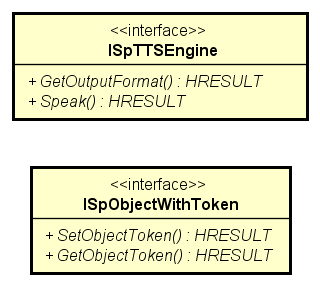
\includegraphics{images/sapi5-interface.png}
	\caption{Interfaccia SAPI~5}
\end{figure}

L'interfaccia SAPI~5 è stata progettata per facilitare il lavoro agli sviluppatori di applicazioni e di engine TTS. Il suo scopo è quello di standardizzare il modo con cui avviene la comunicazione tra applicazioni ed engine TTS. Uno dei task che viene semplificato, utilizzando questa interfaccia, è la gestione del flusso audio. Questo permette agli sviluppatori focalizzarsi maggiormente nello sviluppo dell'engine e non di come il suo output audio venga gestito.
Le interfacce che verranno utilizzate sono ISpTTSEngine e ISpObjectWithToken.
\subsection{ISpObjectWithToken}
L'interfaccia ISpObjectWithToken permette di creare e reperire le informazioni associate ad un oggetto. Nella maggior parte dei casi l'oggetto viene associato ad una voce.
\\\\
\textbf{Metodi}
\begin{itemize}
	\item \texttt{+ SetObjectToken(): HRESULT} imposta le proprietà dell'oggetto passato come parametro.
	\\\\
	\textbf{Argomenti}
	\begin{itemize}
		\item \texttt{pToken: ISpObjectToken} puntatore all'oggetto che deve essere impostato.
	\end{itemize}
	\textbf{Valori di ritorno}
	\begin{itemize}
		\item \texttt{S\_OK} se la funzione non ha generato errori;
		\item \texttt{E\_POINTER} se il parametro \texttt{pToken} non è valido o è malformato;
		\item \texttt{E\_OUTOFMEMORY} se la memoria disponibile non è sufficiente;
		\item \texttt{FAILED(hr)} se c'è un errore da ritornare. 
	\end{itemize}
	
	\item \texttt{+ GetObjectToken(): HRESULT} serve per ottenere un oggetto settato in precedenza. L'oggetto verrà restituito come parametro.
	\\\\
	\textbf{Argomenti}
	\begin{itemize}
		\item \texttt{ppToken: ISpObjectToken} indirizzo dell'oggetto richiesto.
	\end{itemize}
	\textbf{Valori di ritorno}
	\begin{itemize}
		\item \texttt{S\_OK} se la funzione non ha generato errori;
		\item \texttt{E\_POINTER} se il parametro \texttt{ppToken} non è valido o è malformato;
		\item \texttt{E\_OUTOFMEMORY} se la memoria disponibile non è sufficiente;
		\item \texttt{FAILED(hr)} se c'è un errore da ritornare. 
	\end{itemize}
\end{itemize}

\subsection{ISpTTSEngine}
ISpTTSEngine è l'interfaccia principale della specifica SAPI~5. Essa svolge i due compiti principali della sintesi vocale che sono le chiamate all'engine TTS e la generazione dell'audio in un formato specifico. Inoltre gestisce anche gli eventi generati dalla sintesi vocale.
\\\\
\textbf{Metodi}
\begin{itemize}
	\item \texttt{+ GetOutputFormat(): HRESULT} ritorna il formato audio previsto dall'engine TTS;
	\\\\
	\textbf{Argomenti}
	\begin{itemize}
		\item \texttt{pTargetFmtId: GUID} id del formato richiesto come uscita. I valori possibili possono essere di due tipi: \texttt{SPDFID\_Text} per ottenere un formato testuale e \texttt{SPDFID\_WAVEFORMATEX} per un formato audio;
		\item \texttt{pTargetWaveFormatEx: WAVEFORMATEX} se l'identificatore del formato è del tipo \texttt{SPDFID\_WAVEFORMATEX} l'argomento contiene il puntatore alla struttura del formato audio, altrimenti il suo valore è \texttt{NULL};
		\item \texttt{pOutputFormatId: GUID} contiene l'identificatore del formato di uscita che può essere \texttt{SPDFID\_Text} o \texttt{SPDFID\_WAVEFORMATEX}
		\item \texttt{ppCoMemOutputWaveFormatEx: WAVEFORMATEX} contiene la struttura di tipo \texttt{WAVEFORMATEX} del formato audio se l'argomento \texttt{pOutputFormatId} è impostato al valore \texttt{SPDFID\_WAVEFORMATEX} altrimenti è \texttt{NULL}. La struttura verrà allocata tramite \texttt{CoTaskMemAlloc}.
	\end{itemize}
	\item \texttt{+ Speak(): HRESULT} è il metodo che effettua la sintesi vocale trasformando l'input testuale in un formato specifico.
	\\\\
	\textbf{Argomenti}
	\begin{itemize}
		\item \texttt{dwSpeakFlags: DWORD} contiene i valori dei flags che descrivono le caratteristiche dell'input;
		\item \texttt{rguidFormatId: GUID} identificatore del formato di uscita della sintesi vocale. I possibili valori possono essere \texttt{SPDFID\_Text} o \texttt{SPDFID\_WAVEFORMATEX};
		\item \texttt{pWaveFormatEx: WAVEFORMATEX} puntatore alla struttura che descrive il formato d'uscita se il parametro \texttt{rguidFormatId} ha valore \texttt{SPDFID\_WAVEFORMATEX}. L'argomento ha valore \texttt{NULL} se il parametro \texttt{rguidFormatId} ha valore \texttt{SPDFID\_Text};
		\item \texttt{pTextFragList: SPVTEXTFRAG} lista concatenata di \texttt{SPVTEXTFRAG} su cui eseguire la sintesi vocale. Un elemento \texttt{SPVTEXTFRAG} è formato da un frammento di testo decorato da altri atttributi che ne descrivono meglio le caratteristiche;
		\item \texttt{pOutputSite: ISpTTSEngineSite} è il puntatore all'interfaccia \texttt{ISpTTSEngineSite} che viene utilizzato per scrivere l'audio e aggiungere gli eventi SAPI alla coda gestita dall'interfaccia.
	\end{itemize}  
\end{itemize}

\subsection{Descrizione del funzionamento}
Per comprendere al meglio il funzionamento dell'interfaccia SAPI~5 verranno descritte le operazioni che tipicamente vengono eseguite.
Per prima cosa viene effettuata l'inizializzazione dell'engine TTS tramite il metodo \texttt{ISpObjectWithToken::SetObjectToken()}. Questo permette di ottenere un oggetto che può essere utilizzato dall'engine per eseguire la sua inizializzazione.
Ad esempio attraverso questa operazione è possibile impostare la voce con cui verrà effettuata la sintesi vocale.
Una volta che l'engine è stato inizializzato è possibile recuperare le sue informazioni tramite il metodo \texttt{ISpObjectWithToken::GetObjectToken()} e di renderle disponibili, se richieste, ad applicazioni o altri componenti.
Il compito principale di sintesi vocale è affidato al metodo \texttt{ISpTTSEngineSite::Speak()} che si occupa di ricevere l'input testuale, somministrarlo all'engine TTS e scrivere l'output audio in buffer che verrà riprodotto dall'sistema operativo.
Il formato audio che si vuole scrivere deve essere specificato tramite il metodo \texttt{ISpTTSEngineSite::GetOutputFormat()} in modo che l'acquisizione e la riproduzione avvenga nel modo corretto.\\\\
\textbf{Eventi}\\
L'interfaccia SAPI~5 è stata progettata ad eventi e questo comporta che ogni cambiamento di stato sia determinato da un evento.\\
Un evento SAPI è definito da una struttura chiamata \texttt{SPEVENT} che è composta da i seguenti attributi:
\begin{itemize}
	\item \texttt{eEventId: WORD} identifica il tipo di evento tramite un enumeratore;
	\item \texttt{elParamType: WORD} definisce tramite un enumeratore il tipo di \texttt{lParam};
	\item \texttt{ulStreamNum: ULONG} identifica a quale stream appartiene l'evento. Nel nostro caso l'engine TTS non deve preoccuparsi di settare questo parametro, perchè sarà compito dell'applicazione;
	\item \texttt{ullAudioOffset: ULONGLONG} rappresenta l'offset dello stream audio espresso in termini di byte. Buona norma è che questo valore coincida con l'inizio di un campione audio;
	\item \texttt{wParam: WPARAM} è un campo generico che può contenere le informazioni associate all'evento;
	\item \texttt{lParam: LPARAM} è un campo generico che può contenere le informazioni associate all'evento.
\end{itemize}
Adesso andremo ad analizzare gli eventi che possono essere gestiti dall'interfaccia SAPI in base al loro \texttt{eEventId}: 
\begin{description}
	\item [] \texttt{SPEI\_TTS\_BOOKMARK} è l'evento associato al raggiungimento di un \texttt{BOOKMARK}.\\
	I suoi campi generici assumono i seguenti significati:
	\begin{itemize}
		\item \texttt{wParam} contiene la conversione della stringa associata al \texttt{BOOKMARK} nel valore numerico;
		\item \texttt{lParam} contiene la stringa associata al \texttt{BOOKMARK}.
	\end{itemize}
	\item [] \texttt{SPEI\_WORD\_BOUNDARY} è l'evento sollevato in corrispondenza dell'inizio di una parola. Esso viene spesso utilizzato per ottenere l'evidenziazione di una parola sintetizzata in un testo.\\
	I suoi campi generici assumono i seguenti significati:
	\begin{itemize}
		\item \texttt{wParam} rappresenta l'offset espresso in caratteri rispetto all'inizio dell'input;
		\item \texttt{lParam} contiene la lunghezza espressa in caratteri della parola che deve essere sintetizzata.
	\end{itemize}
	\item [] \texttt{SPEI\_SENTENCE\_BOUNDARY} è l'evento sollevato in corrispondenza dell'inizio di una frase.\\
	I suoi campi generici assumono i seguenti significati:
	\begin{itemize}
		\item \texttt{wParam} rappresenta l'offset espresso in caratteri rispetto all'inizio dell'input;
		\item \texttt{lParam} contiene la lunghezza espressa in caratteri della frase che deve essere sintetizzata.
	\end{itemize}
	\item [] \texttt{SPEI\_PHONEME} è l'evento sollevato in corrispondenza della presenza di un fonema. Esso può essere utilizzato per effettuare lo spelling fonetico del testo.\\
	I suoi campi generici assumono i seguenti significati:
	\begin{itemize}
		\item \texttt{wParam} è diviso in due \texttt{WORD}, la \texttt{WORD} più significativa contiene la durata in millisecondi del fonema corrente, invece la \texttt{WORD} meno significativa contiene il \texttt{PhoneID} del fonema successivo;
		\item \texttt{lParam} è diviso in due \texttt{WORD}, la \texttt{WORD} più significativa contiene la \texttt{SPVFEATURE} associata al fonema, invece la \texttt{WORD} meno significativa contiene il \texttt{PhoneID} del fonema corrente.
	\end{itemize}
	\item [] \texttt{SPEI\_VISEME} è l'evento sollevato in corrispondenza della presenza di un visema. Gli eventi di questo tipo possono essere utilizzati per pilotare un avatar.\\
	I suoi campi generici assumono i seguenti significati:
	\begin{itemize}
		\item \texttt{wParam} è diviso in due \texttt{WORD}, la \texttt{WORD} più significativa contiene la durata in millisecondi del visema corrente, invece la \texttt{WORD} meno significativa contiene l'identificatore del visema successivo;
		\item \texttt{lParam} è diviso in due \texttt{WORD}, la \texttt{WORD} più significativa contiene la \texttt{SPVFEATURE} associata al visema, invece la \texttt{WORD} meno significativa contiene l'identificatore del visema corrente.
	\end{itemize}
\end{description}
L'interfaccia SAPI affida la gestione degli eventi ad una coda. Durante la chiamata al metodo \texttt{ISpTTSEngine::Speak()} è possibile eseguire l'inserimento degli eventi nella coda tramite il metodo \texttt{ISpTTSEngineSite::AddEvents()} mediante l'argomento \texttt{pOutputSite}.
L'aspetto più importante è dato dalla relazione che esiste tra lo stream audio e gli eventi. Infatti le due entità vengono trattate come se lo stream audio fosse la linea del tempo e gli eventi degli avvenimenti che accadono in determinato momento identificato dal campo \texttt{ullAudioOffset}.
%immagine linea del tempo con eventi
\\\\
\textbf{Azioni}\\
Lo standard SAPI~5 permette la gestione di azioni che avvengono in tempo reale. Ad esempio è possibile controllare il volume dell'uscita audio o la sua velocità.
Per fare ciò bisogna utilizzare il metodo \texttt{ISpTTSEngineSite::GetActions()} messo a disposizione dall'argomento \texttt{pOutputSite}.
L'invocazione del metodo permette di capire quali azioni sono state effettuate dall'applicazione.Esse possono essere di tre tipi:
\begin{itemize}
	\item \texttt{SPVES\_VOLUME} se il volume è stato cambiato;
	\item \texttt{SPVES\_RATE} se la velocità è stata cambiata;
	\item \texttt{SPVES\_SKIP} se è stata espressa l'intenzione di spostarsi ad un certo punto del testo;
	\item \texttt{SPVES\_ABORT} se la sintesi è stata interrotta;
	\item \texttt{SPVES\_CONTINUE} se nessuna delle precedenti azioni è stata eseguita;
\end{itemize}
Nei i primi tre casi l'interfaccia SAPI mette a disposizione dei metodi per recuperare i nuovi valori e sono rispettivamente:
\begin{itemize}
	\item \texttt{ISpTTSEngineSite::GetVolume(): HRESULT} per recuperare il nuovo valore del volume;
	\item \texttt{ISpTTSEngineSite::GetRate(): HRESULT} per recuperare il nuovo valore della velocità;
	\item \texttt{ISpTTSEngineSite::GetSkipInfo(): HRESULT} per recuperare il tipo e il numero di unità da saltare in avanti o indietro rispetto al punto in cui la sintesi è arrivata. Per completare l'operazione c'è il bisogno di invocare il metodo \texttt{ISpTTSEngineSite::CompleteSkip()} che verifica se è possibile portare a termine l'azione;
\end{itemize}	
Un altro parametro della voce su cui è possibile agire è la tonalità. In questo caso la regolazione non avviene come per la velocità o il volume, ma si deve agire sulla proprietà \texttt{PitchAdj} associata agli elementi della lista \texttt{pTextFragList}.
\section{Implementazione Interfaccia SAPI~5 per MaryTTS}
%\begin{figure}[H]
%	\centering
%	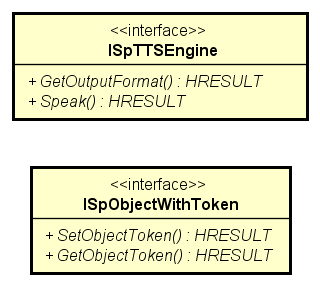
\includegraphics{images/sapi5-interface.png}
%	\caption{Interfaccia SAPI~5}
%\end{figure}
Questa implementazione prevede l'utilizzo dell'engine MaryTTS fornito da Mivoq. L'engine non è disponibile direttamente sottoforma di libreria, ma è integrato in una piattaforma chiamata FA-TTS. Questa piattaforma è scritta in Java ed è essenzialmente un server che risponde alle richieste HTTP in modo REST e nel formato JSON.
Per rendere possibile la comunicazione tra l'implementazione dell'interfaccia SAPI e MaryTTS si è scelto di utilizzare la libreria cURL per eseguire le richieste HTTP al server.
Per gestire in maniera ottimale l'output del server, invece è stata scelta la libreria Jansson che permette di eseguire il parsing degli oggetti JSON.
I compiti a cui dovrà adempire questa implementazione saranno:
\begin{itemize}
	\item richiedere a MaryTTS di eseguire la sintesi vocale dell'input richiesto;
	\item gestire l'output audio e renderlo disponibile al sistema operativo.
	\item eseguire la sintesi vocale con determinati parametri della voce.
\end{itemize}
La forma binaria che assumerà questa implementazione non sarà un'eseguibile ma una libreria dinamica. Questo permetterà al sistema operativo e a tutte le altre applicazioni di poterla utilizzare senza problemi attraverso lo standard SAPI~5.
\subsection{FATTS}
FATTS è la classe che svolge i compiti principali: implementa le interfacce SAPI~5 e dialoga con l'engine MaryTTS tramite la libreria cURL attraverso chiamate HTTP. La parte relativa a SAPI~5 è gestita internamente attraverso i suoi metodi privati, invece la comunicazione con il server è affidata all'entità \texttt{fatts\_client}. FATTS si occupa quindi di gestire gli eventi, le azioni provenienti dalle applicazioni, il formato dell'output e la preparazione dell'input da inviare al server.\\    
\textbf{Implementa:}
\begin{itemize}
	\item \texttt{ISpTTSEngine};
	\item \texttt{ISpTTSObjectWithToken};
\end{itemize}
\textbf{Eredita da:}
\begin{itemize}
	\item \texttt{CComObjectRootEx};
	\item \texttt{CComCoClass};
\end{itemize}
\textbf{Attributi}
\begin{itemize}
	\item \texttt{- voiceToken: CComPtr<ISpObjectToken>} rappresenta l'oggetto che mantiene le informazioni relative alla voce;
	\item \texttt{- voiceProperties: FragmentPropertiesPtr} riferimento ad una mappa che contiene le informazioni relative alla voce in modo centralizzato;
	\item \texttt{- actionAborted: boolean} flag che viene utilizzato per interrompere la sintesi vocale;
	\item \texttt{- actionSkipSentences: int} indica il numero di frasi che la sintesi vocale deve saltare durante l'elaborazione;   
\end{itemize}
\textbf{Metodi}
\begin{itemize}
	\item \texttt{+ FATTS()} è costruttore della classe che serve ad inizializzare le proprietà legate alla voce;
	\item \texttt{+ FinalConstruct(): HRESULT} override del metodo ereditato dalla classe \texttt{CComObjectRootEx} che serve per eseguire le inizializzazioni necessarie dell'oggetto;
	\item \texttt{+ FinalRelease(): void} override del metodo ereditato dalla classe \texttt{CComObjectRootEx} che serve per eseguire la pulizia dell'oggetto prima di distruggerlo;
	\item \texttt{+ SetObjectToken(): HRESULT} metodo che serve per recuperare le informazioni relative alla voce scritte nel registro di Windows. Questo metodo andrà ad impostare l'attributo \texttt{voiceToken}.\\\\
	\textbf{Argomenti}
	\begin{itemize}
		\item \texttt{pToken: ISpObjectToken} è il riferimento al token della voce contenuto nel registro di Windows. 
	\end{itemize}
	\item \texttt{+ GetObjectToken(): HRESULT} metodo che serve per rendere disponibile l'oggetto \texttt{voiceToken} all'esterno;
	\begin{itemize}
		\item \texttt{ppToken: ISpObjectToken} argomento utilizzato per ritornare il l'oggetto impostato tramite il metodo \texttt{SetObjectToken()};
	\end{itemize}
	\item \texttt{Speak(): HRESULT} metodo che serve per effettuare la sintesi vocale attraverso l'engine MaryTTS. Aggiunge gli eventi alla coda e gestisce l'output dell'engine mediante \texttt{pOutputSite}.\\\\
	\textbf{Argomenti}
	\begin{itemize}
		\item \texttt{dwSpeakFlags: DWORD} contiene i valori dei flags che descrivono le caratteristiche dell'input;
		\item \texttt{rguidFormatId: GUID} identificatore del formato di uscita della sintesi vocale. I possibili valori possono essere \texttt{SPDFID\_Text} o \texttt{SPDFID\_WAVEFORMATEX};
		\item \texttt{pWaveFormatEx: WAVEFORMATEX} puntatore alla struttura che descrive il formato d'uscita se il parametro \texttt{rguidFormatId} ha valore \texttt{SPDFID\_WAVEFORMATEX}. L'argomento ha valore \texttt{NULL} se il parametro \texttt{rguidFormatId} ha valore \texttt{SPDFID\_Text};
		\item \texttt{pTextFragList: SPVTEXTFRAG} lista concatenata di \texttt{SPVTEXTFRAG} su cui eseguire la sintesi vocale. Un elemento \texttt{SPVTEXTFRAG} è formato da un frammento di testo decorato da altri atttributi che ne descrivono meglio le caratteristiche;
		\item \texttt{pOutputSite: ISpTTSEngineSite} è il puntatore all'interfaccia \texttt{ISpTTSEngineSite} che viene utilizzato per scrivere l'audio e aggiungere gli eventi SAPI alla coda.
	\end{itemize}
	\item \texttt{+ GetOutputFormat(): HRESULT} ritorna il formato audio previsto dall'engine MaryTTS;
	\\\\
	\textbf{Argomenti}
	\begin{itemize}
		\item \texttt{pTargetFmtId: GUID} id del formato richiesto come uscita. I valori possibili possono essere di due tipi: \texttt{SPDFID\_Text} per ottenere un formato testuale e \texttt{SPDFID\_WAVEFORMATEX} per un formato audio;
		\item \texttt{pTargetWaveFormatEx: WAVEFORMATEX} se l'identificatore del formato è del tipo \texttt{SPDFID\_WAVEFORMATEX} l'argomento contiene il puntatore alla struttura del formato audio, altrimenti il suo valore è \texttt{NULL};
		\item \texttt{pOutputFormatId: GUID} contiene l'identificatore del formato di uscita che può essere \texttt{SPDFID\_Text} o \texttt{SPDFID\_WAVEFORMATEX}
		\item \texttt{ppCoMemOutputWaveFormatEx: WAVEFORMATEX} contiene la struttura di tipo \texttt{WAVEFORMATEX} del formato audio se l'argomento \texttt{pOutputFormatId} è impostato al valore \texttt{SPDFID\_WAVEFORMATEX} altrimenti è \texttt{NULL}. La struttura verrà allocata tramite \texttt{CoTaskMemAlloc}.
	\end{itemize}
	\item \texttt{- ResetActions(): void} metodo che ha il compito di ripristinare l'evoluzione delle azioni compiute allo stato iniziale comportando l'interruzione della sintesi vocale.
	\item \texttt{- HandleActions(): void} metodo che permette di gestire le azioni provenienti dall'applicazione, come la regolazione del volume e della velocità di riproduzione.
	\\\\
	\textbf{Argomenti}
	\begin{itemize}
		\item \texttt{site: ISpTTSEngineSite} riferimento all'interfaccia \texttt{ISpTTSEngineSite} per permettere il recupero delle azioni svolte dall'applicazione;
		\item \texttt{utterance: json\_t} oggetto che rappresenta l'utterance corrente e  viene modificato in base alle azioni che vengono compiute. Ad esempio ad una variazione del volume, l'oggetto in questione viene modificato per permettere la medesima regolazione all'interno dell'engine MaryTTS;
	\end{itemize}
	\item \texttt{- HandleEventInterests(): void} metodo che viene utilizzato all'interno della classe \texttt{FATTS} per capire la tipologia di eventi che vengono sollevati. Questo metodo è utile per variare il comportamento della classe in base agli eventi che si presentano;\\\\
	\textbf{Argomenti}
	\begin{itemize}
		\item \texttt{site: ISpTTSEngineSite} riferimento all'interfaccia \texttt{ISpTTSEngineSite} per permettere la chiamata \texttt{ISpTTSEngineSite::GetEventInterest()} in modo da recuperare la tipologia di eventi sollevata.
	\end{itemize}
	\item \texttt{AdjustProperties(): FragmentPropertiesPtr} metodo che serve per aggiornare le proprietà associate alla voce. L'aggiornamento viene effettuato solamente se sono presenti nuovi valori, altrimenti le proprietà restano invariate.
	\\\\
	\textbf{Argomenti}
	\begin{itemize}
		\item \texttt{state: SPVSTATE} rappresenta l'insieme delle proprietà associate ad un frammento del testo;
		\item \texttt{props: FragmentPropertiesPtr} mappa che contiene le proprietà della voce;
		\item \texttt{utterance: json\_t} oggetto che viene utilizzato da MaryTTS per modificare le caratteristiche della voce durante la sintesi vocale. In particolare, in questo metodo viene utilizzato per modificare la tonalità della voce.
	\end{itemize} 		
\end{itemize}
\subsection{fatts\_client}
\texttt{fatts\_client} è il modulo che comunica direttamente con l'engine MaryTTS attraverso la libreria cURL. L'interazione tra il modulo e MaryTTS avviene mediante richieste HTTP. Invece, per gestire l'output del server in formato JSON si è scelto di utilizzare la libreria Jansson. 
Il modulo si compone di pochi metodi quali l'inizializzazione, la pulizia e la richiesta al server.
Il metodo che effettua la richiesta al server sfrutta il meccanismo delle callback. Infatti gli argomenti del metodo non accettano solo oggetti ma anche funzioni. Questo implica che le callback potranno essere definite all'esterno e assumere vari comportamenti.
\\\\
\textbf{Metodi}
\begin{itemize}
	\item \texttt{fatts\_init(): int} metodo che esegue l'inizializzazione della libreria cURL;
	\item \texttt{fatts\_cleanup(): void} metodo che ha il compito di eseguire la pulizia degli oggetti utilizzati dal client e dalla libreria cURL;
	\item \texttt{fatts\_client\_say\_complete(): int} metodo che esegue la richiesta completa al server. Si occupa di recuperare attraverso l'engine MaryTTS i fonemi, i visemi, le informazioni legate alle parole sintetizzate e il flusso audio da riprodurre.
	Ogni operazione viene effettuata mediante una callback passata come argomento.
	\\\\
	\textbf{Argomenti}
	\begin{itemize}
		\item \texttt{conn: fatts\_client\_s} oggetto che contiene le informazioni relative alla connessione con il server;
		\item \texttt{req : fatts\_request\_s} oggetto che raccoglie tutti i parametri che servono ad effettuare la richiesta al server. I parametri in questione contengono la configurazione della voce, il formato dell'input, l'input testuale e il tipo dell'output desiderato;
		\item \texttt{event\_cb: void} callback utilizzata per aggiungere gli eventi legati ai fonemi e ai visemi alla coda degli eventi tenuta dallo standard SAPI;
		\item \texttt{event\_cb\_data: void} oggetto utilizzato per poter permettere il passaggio dei dati utili alla callback \texttt{event\_cb};
		\item \texttt{word\_event\_cb: void} callback utilizzata per costruire gli eventi legati alle parole da sintetizzare.
		\item \texttt{word\_event\_cb\_data: void} oggetto di supporto utilizzato per rendere possibile il funzionamento della callback \texttt{event\_word\_cb}.
		\item \texttt{write\_callback: size\_t} callback utilizzata per trasferire l'audio proveniente dal server nel buffer che verrà riprodotto.
		\item \texttt{stream: void} rappresenta l'oggetto che verrà utilizzato dalla callback \texttt{write\_callback} per scrivere lo stream audio nel buffer messo a disposizione dallo standard SAPI.
	\end{itemize}
\end{itemize}
\subsection{Descrizione del funzionamento}
Adesso andremo a descrivere il flusso delle operazioni effettuate dall'implementazione con un esempio.
Gli input che l'utente può scegliere tipicamente sono:
\begin{itemize}
	\item la voce;
	\item il testo su cui effettuare la sintesi;
	\item il volume;
	\item la velocità;
	\item la tonalità della voce;
\end{itemize}
Una volta scelti questi parametri è possibile iniziare la sintesi vocale. Ricordiamo che la voce e tutti i suoi parametri sono rappresentati da un token presente nel registro di Windows.
Quindi nel momento della selezione della voce verranno invocati i metodi \texttt{FATTS:SetObjectToken()} e \texttt{FATTS:GetObjectToken()} per rendere disponibile sia all'applicazione sia all'engine MaryTTS le informazioni relative alla voce.
Dopo questa operazione viene invocato il metodo \texttt{FATTS::Speak()} che esegue la sintesi vocale.
All'interno del metodo \texttt{FATTS::Speak()} in un primo momento viene analizzato il testo proveniente dall'applicazione, vengono estratte le proprietà come la tonalità della voce e poi viene ricomposto per essere spedito al server.
Prima di effettuare la richiesta, viene invocato il metodo \texttt{HandleActions()} che permette di recuperare i parametri mancanti come il volume e la velocità e nel medesimo frangente vengono costruiti gli oggetti utili alle callback che avranno il compito di costruire ed aggiungere gli eventi alla coda.
A questo punto il metodo \texttt{fatts\_client\_say\_complete()} è pronto per essere chiamato ed eseguire la richiesta al server.
Il metodo sfruttando la libreria cURL e Jansson elabora l'output del server in formato JSON, esegue la costruzione degli eventi e invia lo stream audio alla riproduzione.

\section{Implementazione Interfaccia SAPI~5 per Speect}
Questa implementazione sfrutta l'engine TTS Speect fornito e sviluppato da Mivoq. Esso è distribuito sottoforma di libreria in modo da permettere il suo utilizzo da parte di altri software.
L'implementazione è analoga a quella usata per MaryTTS. Vengono implementate le interfacce SAPI~5 \texttt{ISpObjectWithToken} e \texttt{ISpTTSEngine}, inoltre vengono ereditate le classi \texttt{CComObjectRootEx} e \texttt{CComCoClass}.
Le classi e i moduli che verranno utilizzati sono: \texttt{SpeectTTS} e \texttt{audio\_event\_functions}.
\texttt{SpeectTTS} ha il compito di implementare i metodi messi a disposizione dall'interfaccia SAPI~5, invece il modulo \texttt{audio\_event\_functions} si preoccupa di interagire con l'engine TTS Speect.
\subsection{SpeectTTS}
La classe \texttt{SpeectTTS} è stata progettata per implementare i metodi dell'interfaccia SAPI~5 e per fornire la struttura minima su cui costruire la libreria dinamica.
Attraverso i suoi metodi inizializza l'engine Speect, ne configura la voce attraverso il metodo \texttt{SpeectTTS::SetObjectToken()} e carica il plugin per gestire lo stream audio.
\texttt{SpeectTTS} inoltre si occupa di gestire le azioni provenienti dall'applicazione e di impostare le proprietà relative alla voce attraverso i metodi \texttt{SpeectTTS::HandleActions()} e \texttt{SpeectTTS::AdjustProperties()}.
Per effettuare la sintesi vocale viene invocato il metodo \texttt{SpeectTTS::Speak()} che attraverso il modulo \texttt{audio\_event\_functions} utilizza l'engine Speect.\\\\
\textbf{Implementa:}
\begin{itemize}
	\item \texttt{ISpObjectWithToken};
	\item \texttt{ISpTTSEngine}.
\end{itemize}
\textbf{Eredita da:}
\begin{itemize}
	\item \texttt{CComObjectRootEx};
	\item \texttt{CComClass}.
\end{itemize}
\textbf{Attributi}
\begin{itemize}
	\item \texttt{- voiceToken: CComPtr<ISpObjectToken>} rappresenta l'oggetto che mantiene le informazioni relative alla voce;
	\item \texttt{- voiceProperties: FragmentPropertiesPtr} riferimento ad una mappa che contiene le informazioni relative alla voce in modo centralizzato;
	\item \texttt{- actionAborted: boolean} flag che viene utilizzato per interrompere la sintesi vocale;
	\item \texttt{- actionSkipSentences: int} indica il numero di frasi che la sintesi vocale deve saltare durante l'elaborazione;
	\item \texttt{- error: s\_erc} oggetto che tiene traccia degli errori di Speect;
	\item \texttt{- riffAudio: SPlugin} rappresenta il plugin che ha il compito di gestire l'output audio di Speect;
	\item \texttt{- voice: SVoice} è l'oggetto che rappresenta la configurazione della voce che utilizzerà Speect per sintetizzare il testo;   
\end{itemize}
\textbf{Metodi}
\begin{itemize}
	\item \texttt{+ SpeectTTS()} è costruttore della classe che serve ad inizializzare le proprietà legate alla voce e gli oggetti che verranno utilizzati da Speect;
	\item \texttt{+ ~SpeectTTS()} è il distruttore della classe e ha il compito di eseguire la pulizia degli oggetti allocati dinamicamente e di Speect; 
	\item \texttt{+ FinalConstruct(): HRESULT} override del metodo ereditato dalla classe \texttt{CComObjectRootEx} che serve per eseguire le inizializzazioni necessarie dell'oggetto;
	\item \texttt{+ FinalRelease(): void} override del metodo ereditato dalla classe \texttt{CComObjectRootEx} che serve per eseguire la pulizia dell'oggetto prima di distruggerlo;
	\item \texttt{+ SetObjectToken(): HRESULT} metodo che serve per recuperare le informazioni relative alla voce scritte nel registro di Windows. Questo metodo andrà ad impostare l'attributo \texttt{voiceToken} e inizializzerà Speect.\\\\
	\textbf{Argomenti}
	\begin{itemize}
		\item \texttt{pToken: ISpObjectToken} è il riferimento al token della voce contenuto nel registro di Windows. 
	\end{itemize}
	\item \texttt{+ GetObjectToken(): HRESULT} metodo che serve per rendere disponibile l'oggetto \texttt{voiceToken} all'esterno;
	\begin{itemize}
		\item \texttt{ppToken: ISpObjectToken} argomento utilizzato per ritornare il l'oggetto impostato tramite il metodo \texttt{SetObjectToken()};
	\end{itemize}
	\item \texttt{Speak(): HRESULT} metodo che serve per effettuare la sintesi vocale attraverso l'engine Speect. Aggiunge gli eventi alla coda e gestisce l'output dell'engine mediante \texttt{pOutputSite}.\\\\
	\textbf{Argomenti}
	\begin{itemize}
		\item \texttt{dwSpeakFlags: DWORD} contiene i valori dei flags che descrivono le caratteristiche dell'input;
		\item \texttt{rguidFormatId: GUID} identificatore del formato di uscita della sintesi vocale. I possibili valori possono essere \texttt{SPDFID\_Text} o \texttt{SPDFID\_WAVEFORMATEX};
		\item \texttt{pWaveFormatEx: WAVEFORMATEX} puntatore alla struttura che descrive il formato d'uscita se il parametro \texttt{rguidFormatId} ha valore \texttt{SPDFID\_WAVEFORMATEX}. L'argomento ha valore \texttt{NULL} se il parametro \texttt{rguidFormatId} ha valore \texttt{SPDFID\_Text};
		\item \texttt{pTextFragList: SPVTEXTFRAG} lista concatenata di \texttt{SPVTEXTFRAG} su cui eseguire la sintesi vocale. Un elemento \texttt{SPVTEXTFRAG} è formato da un frammento di testo decorato da altri atttributi che ne descrivono meglio le caratteristiche;
		\item \texttt{pOutputSite: ISpTTSEngineSite} è il puntatore all'interfaccia \texttt{ISpTTSEngineSite} che viene utilizzato per scrivere l'audio e aggiungere gli eventi SAPI alla coda.
	\end{itemize}
	\item \texttt{+ GetOutputFormat(): HRESULT} ritorna il formato audio previsto dall'engine Speect;
	\\\\
	\textbf{Argomenti}
	\begin{itemize}
		\item \texttt{pTargetFmtId: GUID} id del formato richiesto come uscita. I valori possibili possono essere di due tipi: \texttt{SPDFID\_Text} per ottenere un formato testuale e \texttt{SPDFID\_WAVEFORMATEX} per un formato audio;
		\item \texttt{pTargetWaveFormatEx: WAVEFORMATEX} se l'identificatore del formato è del tipo \texttt{SPDFID\_WAVEFORMATEX} l'argomento contiene il puntatore alla struttura del formato audio, altrimenti il suo valore è \texttt{NULL};
		\item \texttt{pOutputFormatId: GUID} contiene l'identificatore del formato di uscita che può essere \texttt{SPDFID\_Text} o \texttt{SPDFID\_WAVEFORMATEX}
		\item \texttt{ppCoMemOutputWaveFormatEx: WAVEFORMATEX} contiene la struttura di tipo \texttt{WAVEFORMATEX} del formato audio se l'argomento \texttt{pOutputFormatId} è impostato al valore \texttt{SPDFID\_WAVEFORMATEX} altrimenti è \texttt{NULL}. La struttura verrà allocata tramite \texttt{CoTaskMemAlloc}.
	\end{itemize}
	\item \texttt{- ResetActions(): void} metodo che ha il compito di ripristinare l'evoluzione delle azioni compiute allo stato iniziale comportando l'interruzione della sintesi vocale.
	\item \texttt{- HandleActions(): void} metodo che permette di gestire le azioni provenienti dall'applicazione, come la regolazione del volume e della velocità di riproduzione.
	\\\\
	\textbf{Argomenti}
	\begin{itemize}
		\item \texttt{site: ISpTTSEngineSite} riferimento all'interfaccia \texttt{ISpTTSEngineSite} per permettere il recupero delle azioni svolte dall'applicazione;
		\item \texttt{in\_utterance: void} oggetto che rappresenta l'utterance corrente e  viene modificato in base alle azioni che vengono compiute. Ad esempio ad una variazione del volume, l'oggetto in questione viene modificato per permettere la medesima regolazione all'interno dell'engine Speect;
	\end{itemize}
	\item \texttt{- HandleEventInterests(): void} metodo che viene utilizzato all'interno della classe \texttt{SpeectTTS} per capire la tipologia di eventi che vengono sollevati. Questo metodo è utile per variare il comportamento della classe in base agli eventi che si presentano;\\\\
	\textbf{Argomenti}
	\begin{itemize}
		\item \texttt{site: ISpTTSEngineSite} riferimento all'interfaccia \texttt{ISpTTSEngineSite} per permettere la chiamata \texttt{ISpTTSEngineSite::GetEventInterest()} in modo da recuperare la tipologia di eventi sollevata.
	\end{itemize}
	\item \texttt{AdjustProperties(): FragmentPropertiesPtr} metodo che serve per aggiornare le proprietà associate alla voce. L'aggiornamento viene effettuato solamente se sono presenti nuovi valori, altrimenti le proprietà restano invariate.
	\\\\
	\textbf{Argomenti}
	\begin{itemize}
		\item \texttt{state: SPVSTATE} rappresenta l'insieme delle proprietà associate ad un frammento del testo;
		\item \texttt{props: FragmentPropertiesPtr} mappa che contiene le proprietà della voce;
		\item \texttt{utterance: void} oggetto che viene utilizzato da Speect per modificare le caratteristiche della voce durante la sintesi vocale. In particolare, in questo metodo viene utilizzato per modificare la tonalità della voce.
	\end{itemize} 		
\end{itemize}
\subsection{audio\_event\_functions}
\texttt{audio\_event\_functions} è il modulo che si occupa di interagire con l'engine Speect mediante chiamate a funzioni. 
Il metodo principale che compone il modulo è \texttt{speect\_request\_complete\_text()}. I suoi compiti sono: scorrere il grafo Heterogeneous Relation Graph (HRG) presente all'interno di Speect, recuperare le informazioni relative all'input rispetto alle parole e ai fonemi, aggiungere gli eventi SAPI alla coda e scrivere l'audio generato nel buffer gestito da SAPI.
Per adempire ai task relativi allo standard SAPI il modulo \texttt{audio\_event\_functions} fa utilizzo di callback definite nella classe texttt{SpeectTTS}.
\\\\
\textbf{Metodi}
\begin{itemize}
	\item \texttt{speect\_request\_complete\_text(): int} metodo che attraverso l'utilizzo di callback passate come argomento si occupa di gestire gli eventi SAPI relativi alle parole, ai fonemi e ai visemi e di scrivere l'output audio fornito da Speect nel buffer gestito dal sistema operativo.
	\\\\
	\textbf{Argomenti}
	\begin{itemize}
		\item \texttt{input: void} oggetto che contiene i parametri utili a Speect per eseguire la sintesi vocale;
		\item \texttt{event\_cb : void} callback utilizzata per aggiungere gli eventi legati ai fonemi e ai visemi alla coda degli eventi tenuta dallo standard SAPI;
		\item \texttt{event\_cb\_data: void} oggetto utilizzato per poter permettere il passaggio dei dati utili alla callback \texttt{event\_cb};
		\item \texttt{word\_event\_cb: void} callback utilizzata per costruire gli eventi legati alle parole da sintetizzare.
		\item \texttt{word\_event\_cb\_data: void} oggetto di supporto utilizzato per rendere possibile il funzionamento della callback \texttt{event\_word\_cb}.
		\item \texttt{write\_callback: size\_t} callback utilizzata per trasferire l'audio proveniente dal server nel buffer che verrà riprodotto.
		\item \texttt{stream: void} rappresenta l'oggetto che verrà utilizzato dalla callback \texttt{write\_callback} per scrivere lo stream audio nel buffer messo a disposizione dallo standard SAPI.
	\end{itemize}
\end{itemize}
\subsection{Descrizione del funzionamento}
Adesso andremo a descrivere il flusso delle operazioni effettuate dall'implementazione con un esempio.
Gli input che l'utente può scegliere tipicamente sono:
\begin{itemize}
	\item la voce;
	\item il testo su cui effettuare la sintesi;
	\item il volume;
	\item la velocità;
	\item la tonalità della voce;
\end{itemize}
Una volta scelti questi parametri è possibile iniziare la sintesi vocale. Ricordiamo che la voce e tutti i suoi parametri sono rappresentati da un token presente nel registro di Windows.
Quindi nel momento della selezione della voce verranno invocati i metodi \texttt{FATTS:SetObjectToken()} e \texttt{FATTS:GetObjectToken()} per rendere disponibile sia all'applicazione sia all'engine Speect le informazioni relative alla voce.
Dopo questa operazione viene invocato il metodo \texttt{SpeectTTS::Speak()} che esegue la sintesi vocale.
All'interno del metodo \texttt{SpeectTTS::Speak()} in un primo momento viene analizzato il testo proveniente dall'applicazione, vengono estratte le proprietà come la tonalità della voce e poi viene ricomposto per essere processato da Speect.
Prima di eseguire la sintesi, viene invocato il metodo \texttt{HandleActions()} che permette di recuperare i parametri mancanti come il volume e la velocità e nel medesimo frangente vengono costruiti gli oggetti utili alle callback che avranno il compito di costruire ed aggiungere gli eventi alla coda.
A questo punto il metodo \texttt{speect\_request\_complete\_text()} è pronto per essere chiamato ed eseguire la sintesi vocale attraverso Speect.
Durante questa chiamata, Speect scorre le relazioni all'interno del suo Heterogeneous Relation Graph, recuperando le informazioni relative alle parole e ai fonemi. Grazie ad esse riesce attraverso le callback a costruire gli eventi SAPI associati.
Infine Speect mediante il plugin dedicato al rendering audio, genera l'output e attraverso la callback lo carica nel buffer gestito dal sistema operativo.

\section{MaryTTS}
MaryTTS è un engine TTS multilingua open-source sviluppato da DFKI. Dopo aver valutato le sue caratteristiche e funzionalità Mivoq ha scelto di contribuire al suo sviluppo e di integrarlo nella piattaforma FA-TTS.
L'azienda attraverso il suo lavoro ha esteso le funzionalità originali di MaryTTS fornendo nuove API e aggiungendo nuovi formati di input ed output.
La piattaforma FA-TTS, grazie alle conoscenze di Mivoq, può eseguire la sintesi vocale con voci personalizzate, ovvero grazie ad un servizio offerto dall'azienda è possibile creare una voce qualsiasi.
\subsection{Interfaccia Web Client}
La piattaforma FA-TTS è scritta in Java e può essere installata in locale come server.
Dispone di un'interfaccia web molto semplice composta da una casella di testo dove inserire l'input da sintetizzare e delle combo box che servono a selezionare la voce, il tipo di input e il tipo di output desiderati.
Nel caso in cui l'output fosse di tipo audio è possibile selezionare il formato e impostare alcuni effetti audio, tra cui il volume, la tonalità e la velocità della voce.
\subsection{FA-TTS REST API}
La piattaforma FA-TTS mette a disposizione delle API che possono essere interrogate tramite richieste HTTP.
Le API più rilevanti sono:
\begin{itemize}
	\item \textbf{say} viene utilizzata per eseguire la sintesi vocale in base ai parametri richiesti;
	\item \textbf{info/version} serve a recuperare la versione corrente del server;
	\item \textbf{info/voices/all} serve a recuperare tutte le voci disponibili nel server.
\end{itemize}
Adesso andremo ad analizzare degli esempi di richieste utili all'implementazione SAPI per MaryTTS.
\subsubsection{Richiesta stream audio}
Per eseguire la richiesta dello stream audio si utilizza l'API say nella seguente forma:
\lstset{language=html,
		basicstyle=\ttfamily,
		columns=fullflexible,
		showstringspaces=false,
		breaklines=true }
\begin{lstlisting}
http://localhost:59125/say?input[type]=TEXT&input[content]=Benvenuti+nel+mondo+della+sintesi+vocale.&input[locale]=it&output[type]=AUDIO&output[format]=WAVE_FILE&voice[gender]=male&voice[name]=istc-speaker_internazionale-hsmm&voice[age]=35&voice[variant]=1&voice[selection_algorithm]=ssml&utterance[effects]=[{"Volume":1.5},{"F0Add":50.0},{"Rate":3.0}]
\end{lstlisting}
Ad esempio questa richiesta permette di sintetizzare il testo "Benvenuti nel mondo della sintesi vocale" con la voce "istc-speaker\_internazionale-hsmm" di genere maschile con 35 anni.
Sono stati aggiunti anche degli effetti come l'amplificazione del volume, il cambio di tonalità e la diminuzione della velocità.
\subsubsection{Richiesta parole e fonemi}
La seguente richiesta viene impiegata per recuperare le parole e i fonemi sintetizzati da MaryTTS.
\begin{lstlisting}
	http://localhost:59125/say?input[type]=TEXT&input[content]=Benvenuti+nel+mondo+della+sintesi+vocale.&input[locale]=it&output[type]=LIPSYNC&voice[gender]=male&voice[name]=istc-speaker_internazionale-hsmm&voice[age]=35&voice[variant]=1&voice[selection_algorithm]=ssml&utterance[effects]=[{"Volume":1.5},{"F0Add":50.0},{"Rate":3.0}]
\end{lstlisting}
La richiesta è molto simile a quella per recuperare lo stream audio, l'unica differenza è il parametro \texttt{output[type]} impostato con il valore \texttt{LIPSYNC}.\\
La risposta del server è in formato JSON ed è costruita nel seguente modo:
\lstset{language=html,
	basicstyle=\ttfamily,
	columns=fullflexible,
	showstringspaces=false,
	breaklines=true }
\begin{lstlisting}
{
"tokens":[{ 
			"char_end": integer, 
			"start": float,
			"end": float,
			"char_start": integer
}],
"segments":[{ 
			"stressed": boolean, 
			"start": float,
			"end": float,
			"label":  string
}]
}

\end{lstlisting}
L'output è formato da un oggetto composto da due array: \texttt{tokens} e \texttt{segments}.\\
L'array \texttt{tokens} serve a recuperare le informazioni relative alle parole sintetizzate.
Per ogni parola o token è possibile recuperare, grazie a questo array, l'offset espresso in caratteri rispetto all'inizio e alla fine del testo e l'offset espresso in secondi di inizio e fine rispetto allo stream audio.
L'array \texttt{segments} serve per recuperare le informazioni relative ai fonemi sintetizzati.
Per ogni fonema è possibile recuperare l'offset di inizio e fine rispetto allo stream audio, l'etichetta associata al fonema e la proprietà di stress.

\section{Speect}
Speect è un engine TTS multilingua sviluppato dal gruppo Human Language Technologies del Meraka Institute in Sud Africa. 
Mivoq ha scelto di utilizzare questo engine e di portarne avanti lo sviluppo per due motivi essenziali:
\begin{itemize}
	\item Speect è un engine TTS completo e composto interamente da plug-in.Questo favorisce un'alta modularità e aumenta la capacità di testing;
	\item Speect è scritto interamente in C seguendo lo standard ISO/IEC 9899:1990. Questo permette di aver una alta portabilità e compatibilità anche con sistemi non recenti. 
\end{itemize}
La peculiarità di Speect è che il suo funzionamento si basa su una configurazione chiamata voce. Questo permette di scegliere, ad esempio, quali plug-in devo essere abilitati e le caratteristiche che deve avere la sintesi.
Speect può essere utilizzato dalle applicazioni esterne e dai sistemi operativi sottoforma di libreria. Nel caso del sistema operativo Microsoft Windows, Speect viene fornito come libreria dinamica (DLL).
\subsection{Heterogeneous Relation Graph}
Speect per gestire l'analisi testuale sfrutta un grafo chiamato Heterogeneous Relation Graph.
Il grafo ha il compito di tenere traccia delle relazioni che ci sono all'interno del testo.
Le relazioni sono:
\begin{itemize}
	\item \textbf{Phrase} gestisce le relazioni che esistono fra le varie frasi. Tra una frase e l'altra sono presenti due archi, uno punta all'elemento precedente e uno al successivo. Inoltre ogni elemento è il padre del corrispondente elemento nella relazione Word, che da accesso alle singole parole.   
	\item \textbf{Token} gestisce le relazioni che esistono tra i vari tokens. I tokens rappresentano delle unità di testo indivisibili a livello logico.
	Ogni token è collegato tramite due archi, il successivo e il precedente.
	Ogni elemento della relazione è il padre del corrispondente elemento nella relazione Word.
	\item \textbf{Word} gestisce le relazioni che esistono tra le varie parole. Ogni parola è connessa tramite gli archi precedente e successivo.
	\item \textbf{Syllable} gestisce le relazioni tra le varie sillabe. Ogni sillaba è connessa tramite gli archi precedente e successivo.
	\item \textbf{Segment} gestisce le relazioni tra i vari fonemi. Ogni fonema è connesso tramite gli archi precedente e successivo.
	\item \textbf{SylStructure} è l'unione delle relazioni Word, Syllable e Segment, tramite l'arco genitore e figlia.
\end{itemize}
Tutte le relazioni possono essere attraversate orizzontalmente tramite le operazioni "Next" e "Previous".
Solamente le relazioni Phrase, Token e SylStructure possono essere attraversate tramite le operazioni "Parent" e "Daughter".
%immagine grafo HRG
L'attraversamento del grafo HRG è stato utile alla costruzione degli eventi SAPI legati ai fonemi, ai visemi e alle parole
\subsection{Abilitare la serializzazione di un oggetto SAudio in un buffer qualsiasi}
Per soddisfare il requisito \textbf{ob02} è stato necessario introdurre nuovo codice all'interno di Speect.
La necessità di quest'operazione derivava dal fatto che l'engine TTS non era in grado di serializzare un oggetto di tipo \texttt{SAudio} in un buffer.
L'unica funzione a disposizione era \texttt{SObjectSave()} che permetteva di serializzare l'oggetto \texttt{SAudio} come un file dato un percorso.
Per ovviare al problema è stata stata introdotta una nuova classe chiamata \texttt{SGenericsource} e dei nuovi metodi che adesso andremo a descrivere.
\subsubsection{Classe SGenericsource}
La classe \textbf{SGenericsource} estende la classe base \texttt{SDatasource} e ha il compito associare ad un oggetto qualsiasi delle operazioni di input-output, ciò permette la gestione completa del comportamento dell'oggetto.\\\\
\textbf{Eredita da:}
\begin{itemize}
	\item \texttt{SDatasource};
\end{itemize}
\textbf{Attributi}
\begin{itemize}
	\item \texttt{- ptr: void} riferimento all'oggetto generico che deve essere trattato tramite le funzioni di input-output definite all'esterno; 
	\item \texttt{- io\_functs: SIOFunctions} oggetto che contiene le funzioni di input-output definite all'esterno. Le funzioni sono \texttt{read}, \texttt{write}, \texttt{seek} e \texttt{close}.  
\end{itemize}
\textbf{Metodi}
\begin{itemize}
	\item \texttt{+ \_s\_generic\_source\_class\_add(): void} metodo che aggiunge la classe \texttt{SGenericsource} al sistema degli oggetti di Speect.\\
	\textbf{Argomenti}
	\begin{itemize}
		\item \texttt{error: s\_erc} oggetto che tiene traccia degli errori generati da Speect.
	\end{itemize}
	\item \texttt{+ SGenericsourceOpen(): SDatasource} metodo che converte un oggetto qualsiasi nel tipo \texttt{SDatasource}. Assieme all'oggetto devono essere fornite anche le funzioni di input-output.\\
	\textbf{Argomenti}
	\begin{itemize}
		\item \texttt{ptr: void} oggetto che deve essere interpretato come \texttt{SDatasource};
		\item \texttt{mode: char} stringa che indica in quale modalità deve essere trattato l'oggetto;
		\item \texttt{io\_functs: SIOFunctions} oggetto che raccoglie le funzioni di input e output che servono ad eseguire le operazioni sull'oggetto \texttt{ptr};
		\item \texttt{error: s\_erc} oggetto che tiene traccia degli errori generati da Speect.
	\end{itemize} 
\end{itemize}

\subsubsection{Modulo serialize}
Il modulo \texttt{serialize} è una raccolta di funzioni che si occupa della serializzazione degli oggetti trattati da Speect attraverso l'Object System.
Per soddisfare il requisito \textbf{ob02} c'è stato il bisogno di introdurre un nuovo metodo chiamato \texttt{SObjectSaveToDatasource()}.\\\\
\textbf{Metodi:}
\begin{itemize}
	\item \texttt{+ SObjectSaveToDatasource(): void} serve a serializzare un oggetto che appartiene all'Object System di Speect in un oggetto di tipo \texttt{SDatasource}.\\\\
	\textbf{Argomenti}
	\begin{itemize}
		\item \texttt{object: SObject} oggetto che deve essere serializzato;
		\item \texttt{ds: SDatasource} destinazione della serializzazione dell'oggetto;
		\item \texttt{format: char} formato di destinazione dell'oggetto che deve essere serializzato;
		\item \texttt{error: s\_erc} oggetto che traccia gli errori generati da Speect.
	\end{itemize}
\end{itemize}

\subsubsection{Classe SSerializedFileClass}
\texttt{SSerializedFileClass} è una classe astratta che estende \texttt{SObjectClass} e viene utilizzata per trattare i file e le sue operazioni di input e output.
In origine la classe permetteva tramite una sua estensione concreta di serializzare un oggetto solo in un percorso. Per ovviare a questa limitazione si è scelto di introdurre un nuovo metodo chiamato SSerializedFileSaveToDatasource().\\\\
\textbf{Eredita da:}
\begin{itemize}
	\item \texttt{SObjectClass}.
\end{itemize}
\textbf{Metodi:}
\begin{itemize}
	\item \texttt{+ SSerializedFileSaveToDatasource(): void} serve a serializzare un oggetto che appartiene all'Object System di Speect in un oggetto di tipo \texttt{SDatasource}.\\
	\textbf{Argomenti}
	\begin{itemize}
		\item \texttt{self: SSerializedFile} oggetto che viene utilizzato come riferimento in terno per invocare i metodi della classe; 
		\item \texttt{object: SObject} oggetto che deve essere serializzato;
		\item \texttt{ds: SDatasource} destinazione della serializzazione dell'oggetto;
		\item \texttt{format: char} formato di destinazione dell'oggetto che deve essere serializzato;
		\item \texttt{error: s\_erc} oggetto che traccia gli errori generati da Speect.
	\end{itemize}
\end{itemize}
 
\subsubsection{Classe SRIFFAudioFileClass}
La classe \texttt{SRIFFAudioFileClass} è un'estensione concreta della classe astratta \texttt{SSerializedFileClass} e ha il compito di serializzare un oggetto di tipo \texttt{SAudio} nel formato riff.
Per permettere la serializzazione verso un oggetto di tipo \texttt{SDatasource} è stato aggiunto un nuovo metodo chiamato \texttt{SaveToDatasource()}.\\\\
\textbf{Eredita da:}
\begin{itemize}
	\item \texttt{SSerializedFileClass}.
\end{itemize}
\textbf{Metodi}
\begin{itemize}
	\item \texttt{+ SaveToDatasource(): void} serve a serializzare un oggetto di tipo \texttt{SAudio} in un oggetto di tipo \texttt{SDatasource}.\\\\
	\textbf{Argomenti}
	\begin{itemize}
		\item \texttt{object: SObject} oggetto che deve essere serializzato;
		\item \texttt{ds: SDatasource} destinazione della serializzazione dell'oggetto;
		\item \texttt{error: s\_erc} oggetto che traccia gli errori generati da Speect.
	\end{itemize}
\end{itemize}

\subsubsection{Modulo write}
Il modulo \texttt{write} fornisce delle funzioni di supporto alla classe \texttt{SRIFFAudioFileClass}. Per implementare il metodo \texttt{SRIFFAudioFileClass::SaveToDatasource()} è stato necessario aggiungere un nuovo metodo al modulo \texttt{write} chiamato \texttt{s\_write\_audio\_riff\_16\_to\_datasource()}.\\\\
\textbf{Metodi}
\begin{itemize}
	\item \texttt{+ s\_write\_audio\_riff\_16\_to\_datasource(): void} serve a serializzare un oggetto di tipo \texttt{SAudio} in un oggetto di tipo \texttt{SDatasource}.\\\\
	\textbf{Argomenti}
	\begin{itemize}
		\item \texttt{object: SObject} oggetto che deve essere serializzato;
		\item \texttt{ds: SDatasource} destinazione della serializzazione dell'oggetto;
		\item \texttt{error: s\_erc} oggetto che traccia gli errori generati da Speect.
	\end{itemize}
\end{itemize}

\subsection{Aggiunta feature cambio volume, velocità e tonalità}
Speect, come richiesto dal requisito \textbf{de01}, deve supportare il cambio di velocità e di tonalità della voce. 
Per soddisfare questo requisito è stato necessario introdurre dei nuovi metodi all'interno del plugin che gestisce l'output audio.
Il plugin in questione utilizza le API HTS\_engine 1.05 che sono in grado di generare e gestire uno stream audio.\\
Di seguito andremo ad analizzare i metodi che sono stati aggiunti.\\\\
\textbf{Metodi:}
\begin{itemize}
	\item \texttt{check\_and\_change\_rate\_volume()} serve a modificare il volume o la velocità della voce se è stato rilevato un cambiamento;\\\\
	\textbf{Argomenti}
	\begin{itemize}
		\item \texttt{HTSsynth: SHTSEngineSynthUttProc105} oggetto che rappresenta l'Utterance Processor associato al plugin che utilizza le API HTS\_engine 1.05;
		\item \texttt{utt: SUtterance} oggetto che rappresenta l'Utterance associata alla sintesi corrente;
		\item \texttt{error: s\_erc} oggetto che tiene traccia degli errori di Speect.
	\end{itemize}
	\item \texttt{check\_and\_change\_tone()} serve a modificare la tonalità della voce se è stato rilevato un cambiamento;\\\\
	\textbf{Argomenti}
	\begin{itemize}
		\item \texttt{HTSsynth: SHTSEngineSynthUttProc105} oggetto che rappresenta l'Utterance Processor associato al plugin che utilizza le API HTS\_engine 1.05;
		\item \texttt{utt: SUtterance} oggetto che rappresenta l'Utterance associata alla sintesi corrente;
		\item \texttt{error: s\_erc} oggetto che tiene traccia degli errori di Speect.
	\end{itemize}
\end{itemize}

